\documentclass[12pt]{article}
\usepackage[letterpaper, left=12mm, right=12mm, top=17mm, bottom=17mm,
            headheight=6mm, headsep=5mm, footskip=9mm]{geometry}
\usepackage[T1]{fontenc}
\usepackage{tgheros}
\renewcommand{\familydefault}{\sfdefault}
\usepackage{tikz}
\usepackage{pifont}
\usepackage{fancyhdr}
\pagestyle{fancy}
\fancyhf{}
\fancyhead[L]{Week 98 / Growing from a few seeds / K--1}
\fancyfoot[L]{\small Bellingham Math Circle / Week 98 / W98-K-v1}
\fancyfoot[R]{\small \thepage}
\renewcommand{\headrulewidth}{0.4pt}
\setlength{\parindent}{0pt}
\setlength{\parskip}{0pt}
\raggedright
\begin{document}
\noindent\begin{minipage}[t]{97mm}\vspace{0pt}\raggedright\setlength{\parskip}{0pt}
Seeds are the first counters on a board, all in one color. Grow the board with counters of the other color. A square gets a counter when two or more squares next to it, not corner to corner, have counters. Your partner points to two of them before each new counter. Counters stay put. When no square can get a counter, the board is filled or stuck.
\end{minipage}\hfill\begin{minipage}[t]{91.0mm}\vspace{1mm}\raggedleft
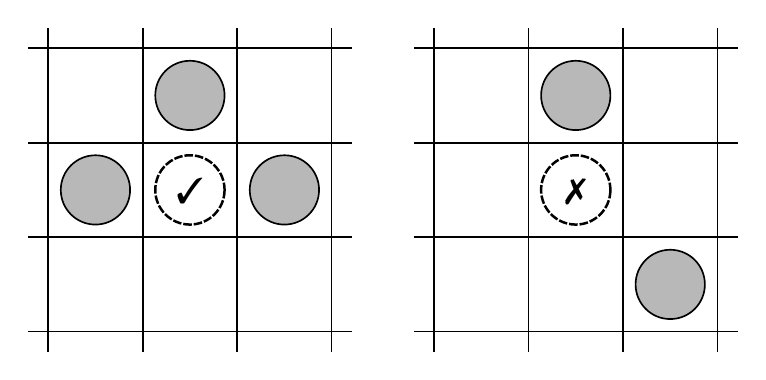
\begin{tikzpicture}[x=1mm,y=1mm,line cap=rect]
\draw[line width=0.6pt] (2.5,2.5) -- (2.5,-38.5);
\draw[line width=0.6pt] (0.0,0) -- (41.0,0);
\draw[line width=0.6pt] (14.5,2.5) -- (14.5,-38.5);
\draw[line width=0.6pt] (0.0,-12) -- (41.0,-12);
\draw[line width=0.6pt] (26.5,2.5) -- (26.5,-38.5);
\draw[line width=0.6pt] (0.0,-24) -- (41.0,-24);
\draw[line width=0.6pt] (38.5,2.5) -- (38.5,-38.5);
\draw[line width=0.6pt] (0.0,-36) -- (41.0,-36);
\filldraw[fill=black!28, draw=black, line width=0.6pt] (20.50,-6.00) circle (4.4);
\filldraw[fill=black!28, draw=black, line width=0.6pt] (8.50,-18.00) circle (4.4);
\filldraw[fill=black!28, draw=black, line width=0.6pt] (32.50,-18.00) circle (4.4);
\draw[line width=0.9pt, dash pattern=on 2.2pt off 1.6pt] (20.50,-18.00) circle (4.4);
\node at (20.50,-18.20) {\fontsize{13}{14}\selectfont \ding{51}};
\draw[line width=0.6pt] (51.5,2.5) -- (51.5,-38.5);
\draw[line width=0.6pt] (49.0,0) -- (90.0,0);
\draw[line width=0.6pt] (63.5,2.5) -- (63.5,-38.5);
\draw[line width=0.6pt] (49.0,-12) -- (90.0,-12);
\draw[line width=0.6pt] (75.5,2.5) -- (75.5,-38.5);
\draw[line width=0.6pt] (49.0,-24) -- (90.0,-24);
\draw[line width=0.6pt] (87.5,2.5) -- (87.5,-38.5);
\draw[line width=0.6pt] (49.0,-36) -- (90.0,-36);
\filldraw[fill=black!28, draw=black, line width=0.6pt] (69.50,-6.00) circle (4.4);
\filldraw[fill=black!28, draw=black, line width=0.6pt] (81.50,-30.00) circle (4.4);
\draw[line width=0.9pt, dash pattern=on 2.2pt off 1.6pt] (69.50,-18.00) circle (4.4);
\node at (69.50,-18.20) {\fontsize{13}{14}\selectfont \ding{55}};
\end{tikzpicture}
\end{minipage}\par\vspace{10mm}
\textbf{Problem 1:} Find every way to put 2 seeds on this board. Draw each way with dots, and ring the ways that fill.\par\vspace{5mm}
\noindent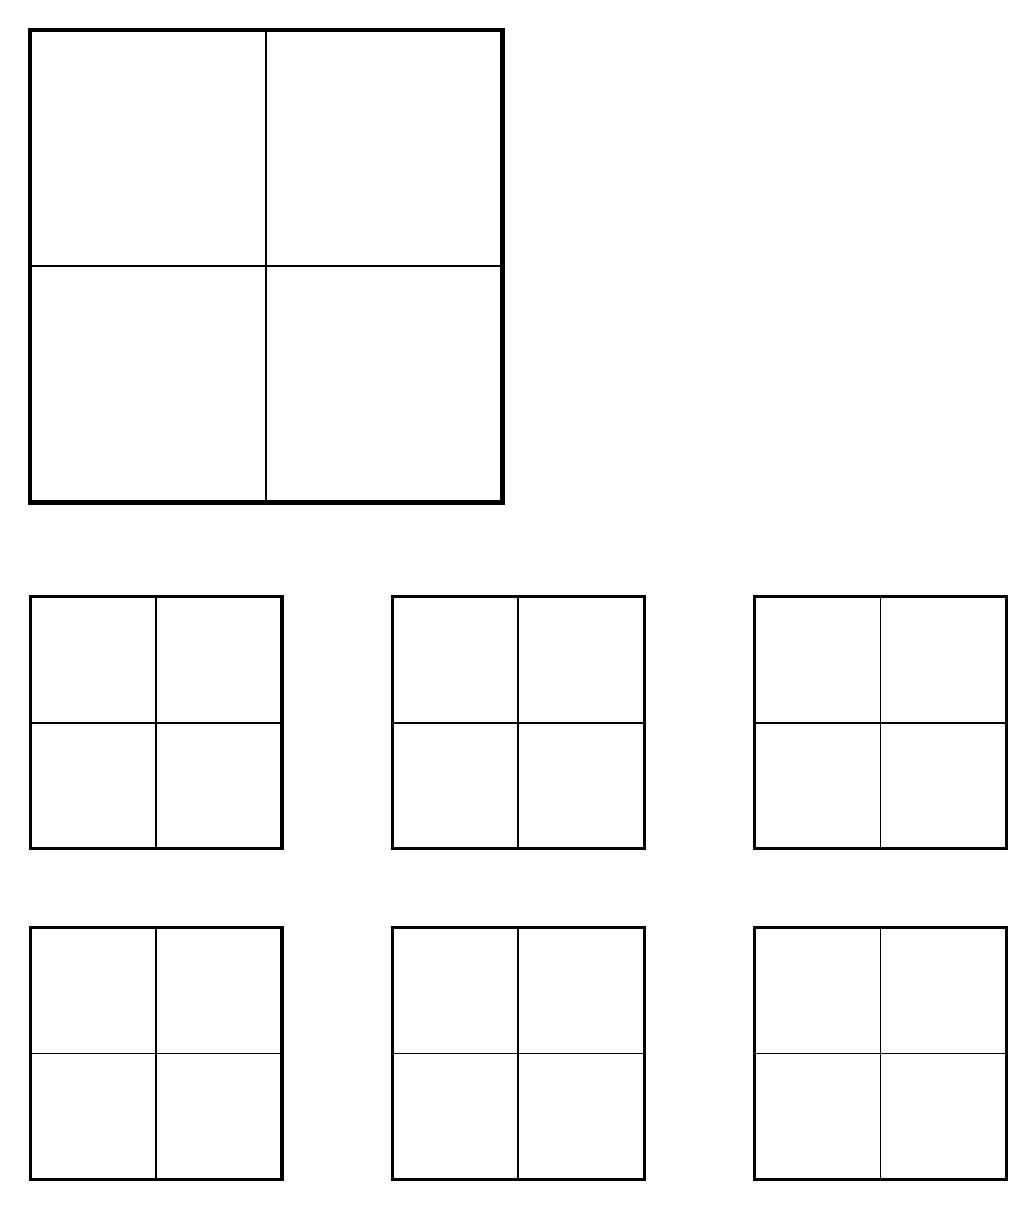
\begin{tikzpicture}[x=1mm,y=1mm,line cap=rect]
\draw[line width=0.9pt] (30,0) -- (30,-60);
\draw[line width=0.9pt] (0,-30) -- (60,-30);
\draw[line width=1.7pt] (0,0) rectangle (60,-60);
\draw[line width=0.6pt] (16,-72) -- (16,-104);
\draw[line width=0.6pt] (0,-88) -- (32,-88);
\draw[line width=1.1pt] (0,-72) rectangle (32,-104);
\draw[line width=0.6pt] (62,-72) -- (62,-104);
\draw[line width=0.6pt] (46,-88) -- (78,-88);
\draw[line width=1.1pt] (46,-72) rectangle (78,-104);
\draw[line width=0.6pt] (108,-72) -- (108,-104);
\draw[line width=0.6pt] (92,-88) -- (124,-88);
\draw[line width=1.1pt] (92,-72) rectangle (124,-104);
\draw[line width=0.6pt] (16,-114) -- (16,-146);
\draw[line width=0.6pt] (0,-130) -- (32,-130);
\draw[line width=1.1pt] (0,-114) rectangle (32,-146);
\draw[line width=0.6pt] (62,-114) -- (62,-146);
\draw[line width=0.6pt] (46,-130) -- (78,-130);
\draw[line width=1.1pt] (46,-114) rectangle (78,-146);
\draw[line width=0.6pt] (108,-114) -- (108,-146);
\draw[line width=0.6pt] (92,-130) -- (124,-130);
\draw[line width=1.1pt] (92,-114) rectangle (124,-146);
\end{tikzpicture}

\newpage
\textbf{Problem 2:} Which of these boards can still grow? Grow each one until it stops.\par\vspace{5mm}
\noindent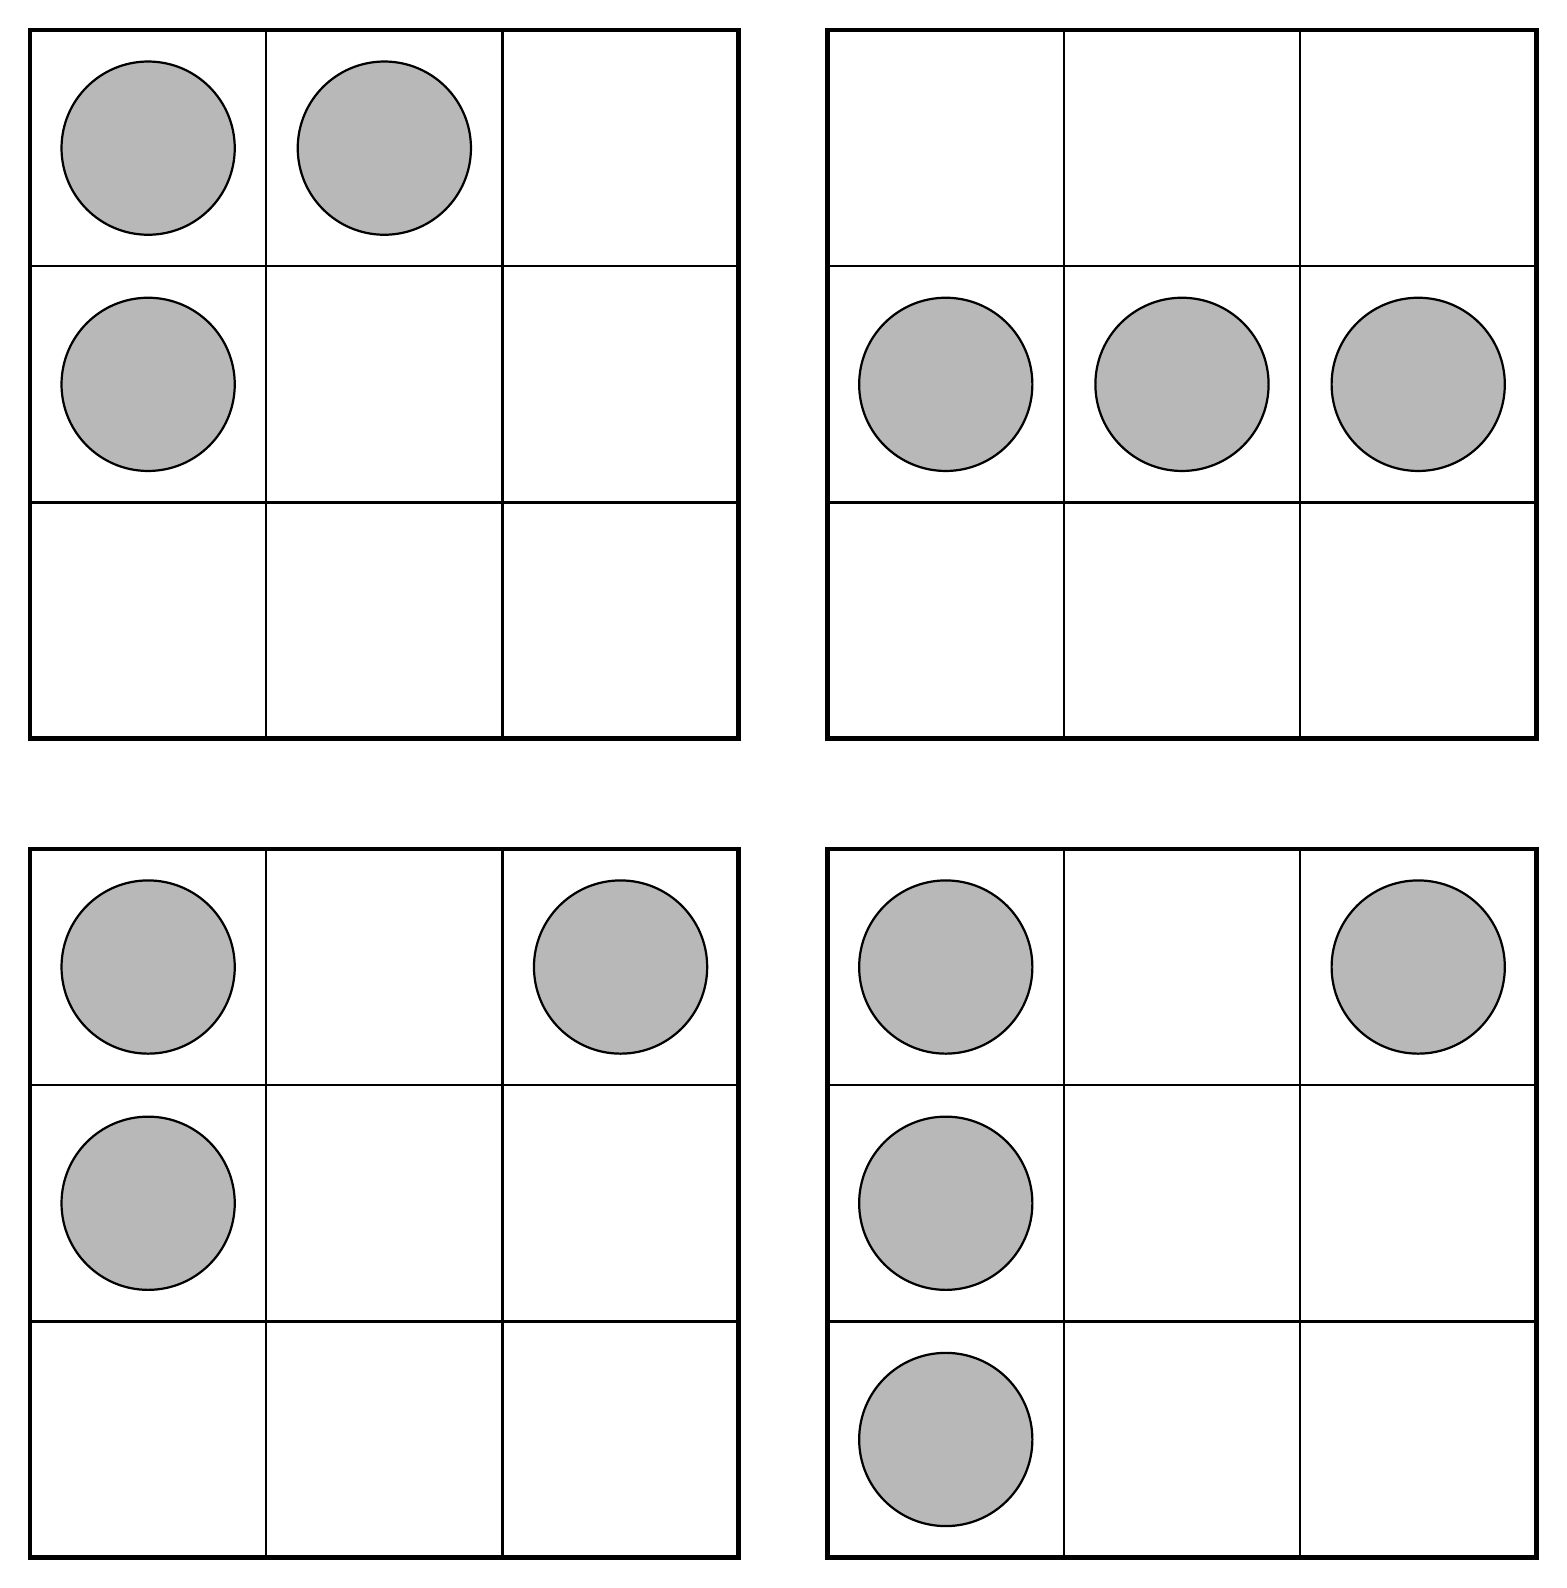
\begin{tikzpicture}[x=1mm,y=1mm,line cap=rect]
\draw[line width=0.9pt] (30.0,0) -- (30.0,-90);
\draw[line width=0.9pt] (60.0,0) -- (60.0,-90);
\draw[line width=0.9pt] (0.0,-30) -- (90.0,-30);
\draw[line width=0.9pt] (0.0,-60) -- (90.0,-60);
\draw[line width=1.7pt] (0.0,0) rectangle (90.0,-90);
\filldraw[fill=black!28, draw=black, line width=0.8pt] (15.00,-15.00) circle (11);
\filldraw[fill=black!28, draw=black, line width=0.8pt] (45.00,-15.00) circle (11);
\filldraw[fill=black!28, draw=black, line width=0.8pt] (15.00,-45.00) circle (11);
\draw[line width=0.9pt] (131.3,0) -- (131.3,-90);
\draw[line width=0.9pt] (161.3,0) -- (161.3,-90);
\draw[line width=0.9pt] (101.30000000000001,-30) -- (191.3,-30);
\draw[line width=0.9pt] (101.30000000000001,-60) -- (191.3,-60);
\draw[line width=1.7pt] (101.30000000000001,0) rectangle (191.3,-90);
\filldraw[fill=black!28, draw=black, line width=0.8pt] (116.30,-45.00) circle (11);
\filldraw[fill=black!28, draw=black, line width=0.8pt] (146.30,-45.00) circle (11);
\filldraw[fill=black!28, draw=black, line width=0.8pt] (176.30,-45.00) circle (11);
\draw[line width=0.9pt] (30.0,-104) -- (30.0,-194);
\draw[line width=0.9pt] (60.0,-104) -- (60.0,-194);
\draw[line width=0.9pt] (0.0,-134) -- (90.0,-134);
\draw[line width=0.9pt] (0.0,-164) -- (90.0,-164);
\draw[line width=1.7pt] (0.0,-104) rectangle (90.0,-194);
\filldraw[fill=black!28, draw=black, line width=0.8pt] (15.00,-119.00) circle (11);
\filldraw[fill=black!28, draw=black, line width=0.8pt] (75.00,-119.00) circle (11);
\filldraw[fill=black!28, draw=black, line width=0.8pt] (15.00,-149.00) circle (11);
\draw[line width=0.9pt] (131.3,-104) -- (131.3,-194);
\draw[line width=0.9pt] (161.3,-104) -- (161.3,-194);
\draw[line width=0.9pt] (101.30000000000001,-134) -- (191.3,-134);
\draw[line width=0.9pt] (101.30000000000001,-164) -- (191.3,-164);
\draw[line width=1.7pt] (101.30000000000001,-104) rectangle (191.3,-194);
\filldraw[fill=black!28, draw=black, line width=0.8pt] (116.30,-119.00) circle (11);
\filldraw[fill=black!28, draw=black, line width=0.8pt] (116.30,-149.00) circle (11);
\filldraw[fill=black!28, draw=black, line width=0.8pt] (116.30,-179.00) circle (11);
\filldraw[fill=black!28, draw=black, line width=0.8pt] (176.30,-119.00) circle (11);
\end{tikzpicture}

\newpage
\textbf{Problem 3:} Fill this board with as few seeds as you can, and draw the seeds.\par\vspace{5mm}
\noindent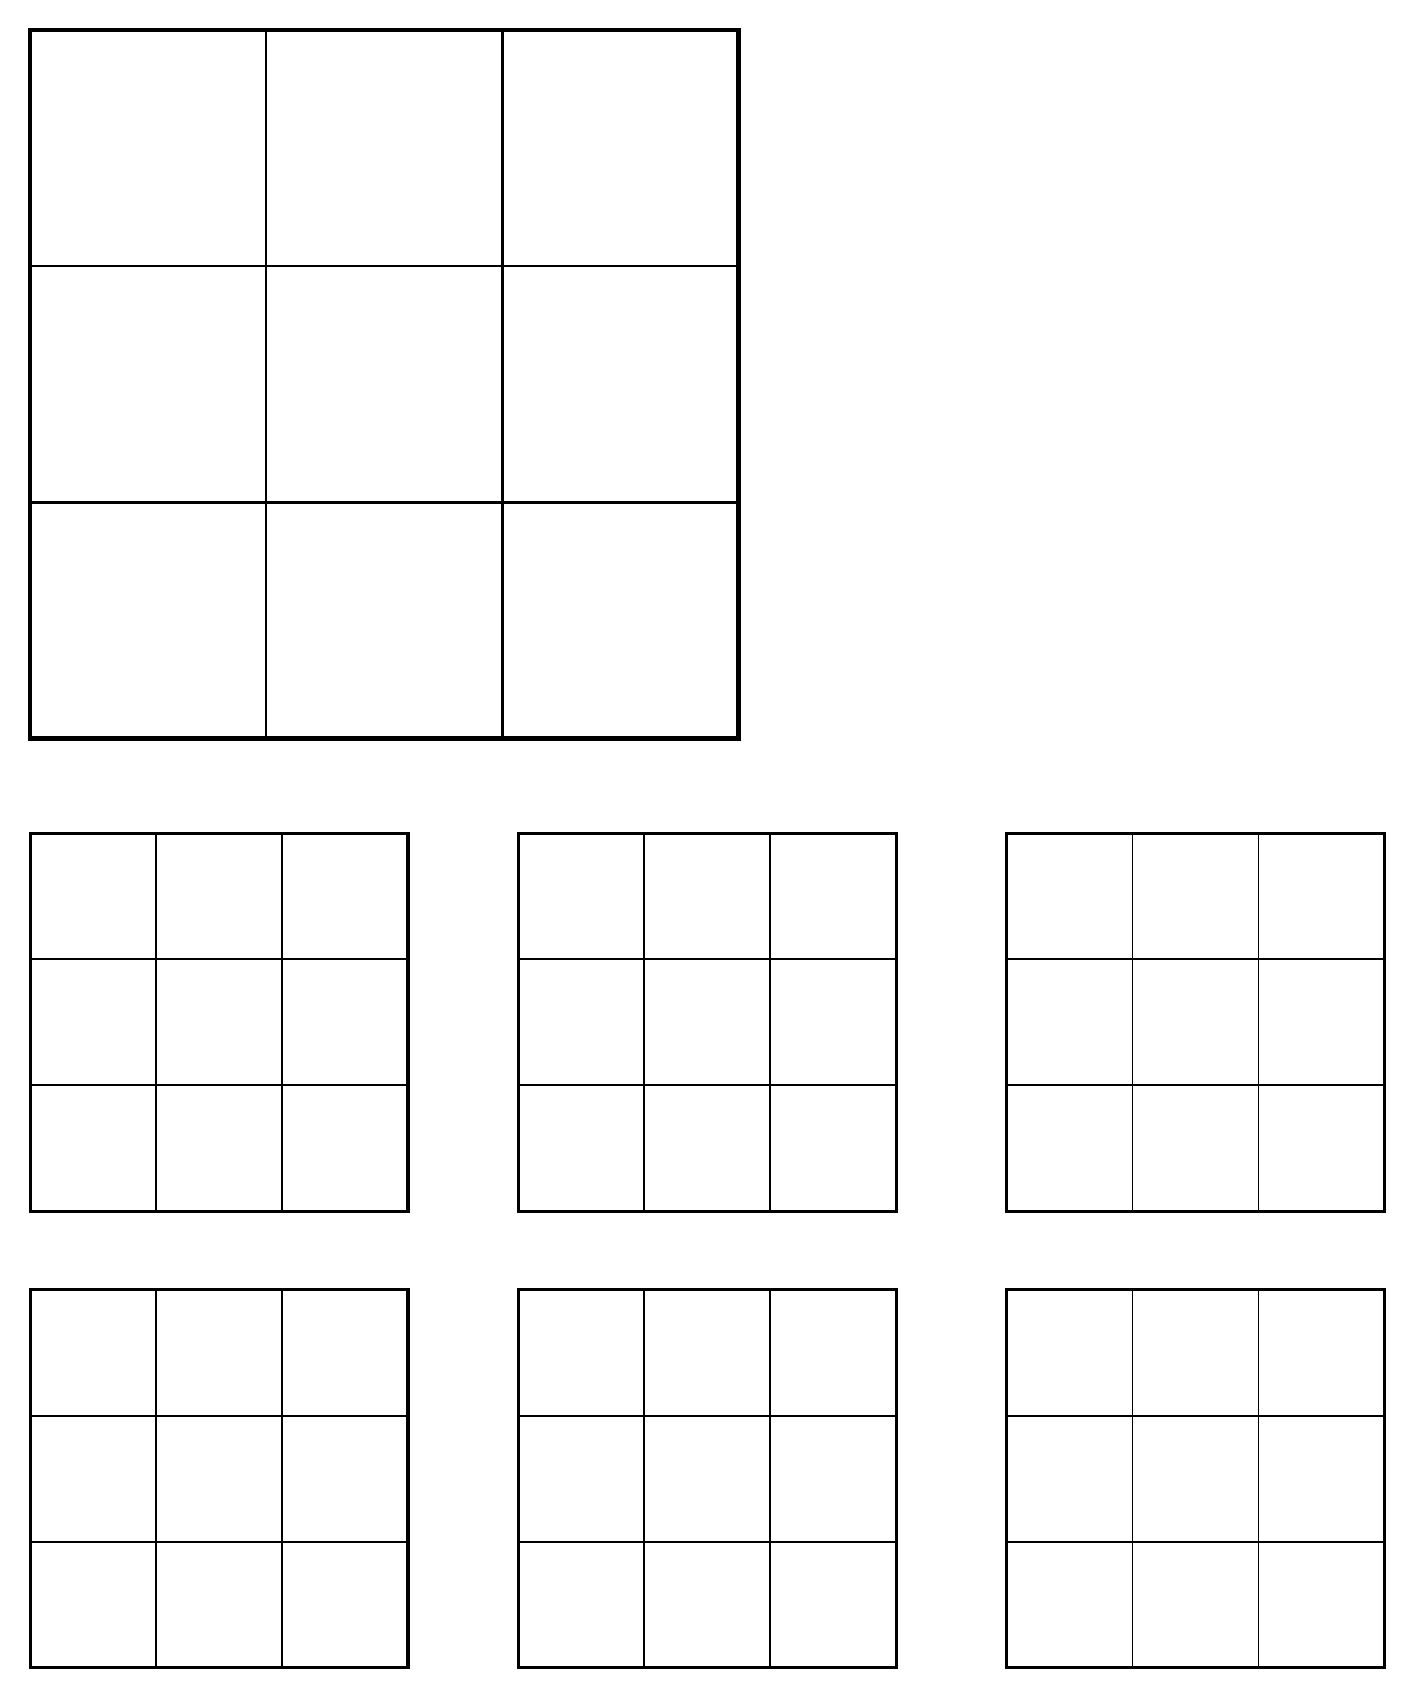
\begin{tikzpicture}[x=1mm,y=1mm,line cap=rect]
\draw[line width=0.9pt] (30,0) -- (30,-90);
\draw[line width=0.9pt] (60,0) -- (60,-90);
\draw[line width=0.9pt] (0,-30) -- (90,-30);
\draw[line width=0.9pt] (0,-60) -- (90,-60);
\draw[line width=1.7pt] (0,0) rectangle (90,-90);
\draw[line width=0.6pt] (16,-102) -- (16,-150);
\draw[line width=0.6pt] (32,-102) -- (32,-150);
\draw[line width=0.6pt] (0,-118) -- (48,-118);
\draw[line width=0.6pt] (0,-134) -- (48,-134);
\draw[line width=1.1pt] (0,-102) rectangle (48,-150);
\draw[line width=0.6pt] (78,-102) -- (78,-150);
\draw[line width=0.6pt] (94,-102) -- (94,-150);
\draw[line width=0.6pt] (62,-118) -- (110,-118);
\draw[line width=0.6pt] (62,-134) -- (110,-134);
\draw[line width=1.1pt] (62,-102) rectangle (110,-150);
\draw[line width=0.6pt] (140,-102) -- (140,-150);
\draw[line width=0.6pt] (156,-102) -- (156,-150);
\draw[line width=0.6pt] (124,-118) -- (172,-118);
\draw[line width=0.6pt] (124,-134) -- (172,-134);
\draw[line width=1.1pt] (124,-102) rectangle (172,-150);
\draw[line width=0.6pt] (16,-160) -- (16,-208);
\draw[line width=0.6pt] (32,-160) -- (32,-208);
\draw[line width=0.6pt] (0,-176) -- (48,-176);
\draw[line width=0.6pt] (0,-192) -- (48,-192);
\draw[line width=1.1pt] (0,-160) rectangle (48,-208);
\draw[line width=0.6pt] (78,-160) -- (78,-208);
\draw[line width=0.6pt] (94,-160) -- (94,-208);
\draw[line width=0.6pt] (62,-176) -- (110,-176);
\draw[line width=0.6pt] (62,-192) -- (110,-192);
\draw[line width=1.1pt] (62,-160) rectangle (110,-208);
\draw[line width=0.6pt] (140,-160) -- (140,-208);
\draw[line width=0.6pt] (156,-160) -- (156,-208);
\draw[line width=0.6pt] (124,-176) -- (172,-176);
\draw[line width=0.6pt] (124,-192) -- (172,-192);
\draw[line width=1.1pt] (124,-160) rectangle (172,-208);
\end{tikzpicture}

\newpage
\textbf{Problem 4:} Guess how few seeds can fill this board. Then fill it with as few seeds as you can, and draw the seeds.\par\vspace{5mm}
\noindent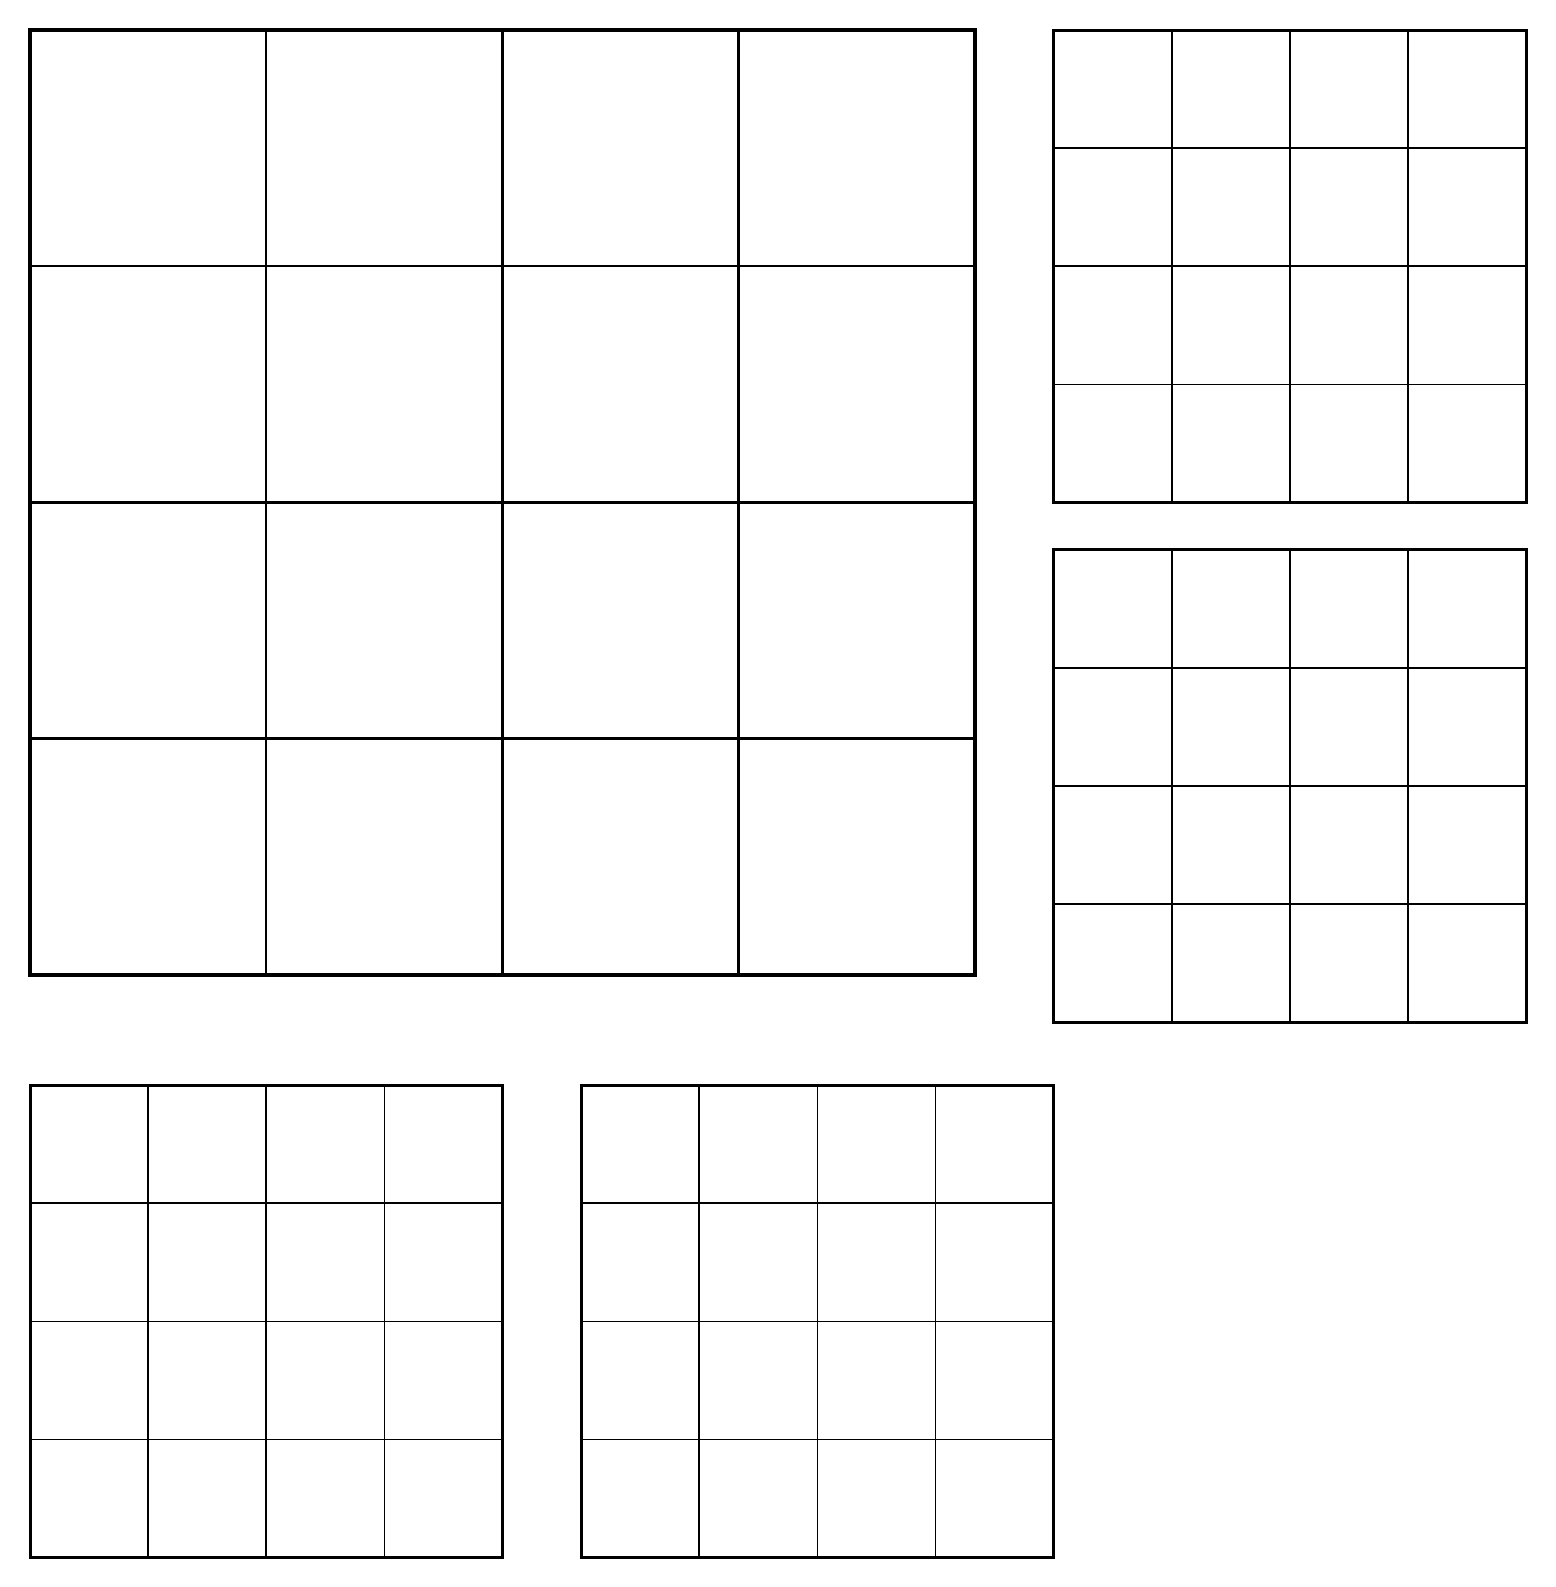
\begin{tikzpicture}[x=1mm,y=1mm,line cap=rect]
\draw[line width=0.9pt] (30,0) -- (30,-120);
\draw[line width=0.9pt] (60,0) -- (60,-120);
\draw[line width=0.9pt] (90,0) -- (90,-120);
\draw[line width=0.9pt] (0,-30) -- (120,-30);
\draw[line width=0.9pt] (0,-60) -- (120,-60);
\draw[line width=0.9pt] (0,-90) -- (120,-90);
\draw[line width=1.7pt] (0,0) rectangle (120,-120);
\draw[line width=0.6pt] (145,0) -- (145,-60);
\draw[line width=0.6pt] (160,0) -- (160,-60);
\draw[line width=0.6pt] (175,0) -- (175,-60);
\draw[line width=0.6pt] (130,-15) -- (190,-15);
\draw[line width=0.6pt] (130,-30) -- (190,-30);
\draw[line width=0.6pt] (130,-45) -- (190,-45);
\draw[line width=1.1pt] (130,0) rectangle (190,-60);
\draw[line width=0.6pt] (145,-66) -- (145,-126);
\draw[line width=0.6pt] (160,-66) -- (160,-126);
\draw[line width=0.6pt] (175,-66) -- (175,-126);
\draw[line width=0.6pt] (130,-81) -- (190,-81);
\draw[line width=0.6pt] (130,-96) -- (190,-96);
\draw[line width=0.6pt] (130,-111) -- (190,-111);
\draw[line width=1.1pt] (130,-66) rectangle (190,-126);
\draw[line width=0.6pt] (15,-134) -- (15,-194);
\draw[line width=0.6pt] (30,-134) -- (30,-194);
\draw[line width=0.6pt] (45,-134) -- (45,-194);
\draw[line width=0.6pt] (0,-149) -- (60,-149);
\draw[line width=0.6pt] (0,-164) -- (60,-164);
\draw[line width=0.6pt] (0,-179) -- (60,-179);
\draw[line width=1.1pt] (0,-134) rectangle (60,-194);
\draw[line width=0.6pt] (85,-134) -- (85,-194);
\draw[line width=0.6pt] (100,-134) -- (100,-194);
\draw[line width=0.6pt] (115,-134) -- (115,-194);
\draw[line width=0.6pt] (70,-149) -- (130,-149);
\draw[line width=0.6pt] (70,-164) -- (130,-164);
\draw[line width=0.6pt] (70,-179) -- (130,-179);
\draw[line width=1.1pt] (70,-134) rectangle (130,-194);
\end{tikzpicture}

\newpage
\textbf{Problem 5:} Guess how few seeds can fill this board. Then fill it with as few seeds as you can, and draw the seeds.\par\vspace{3mm}
\noindent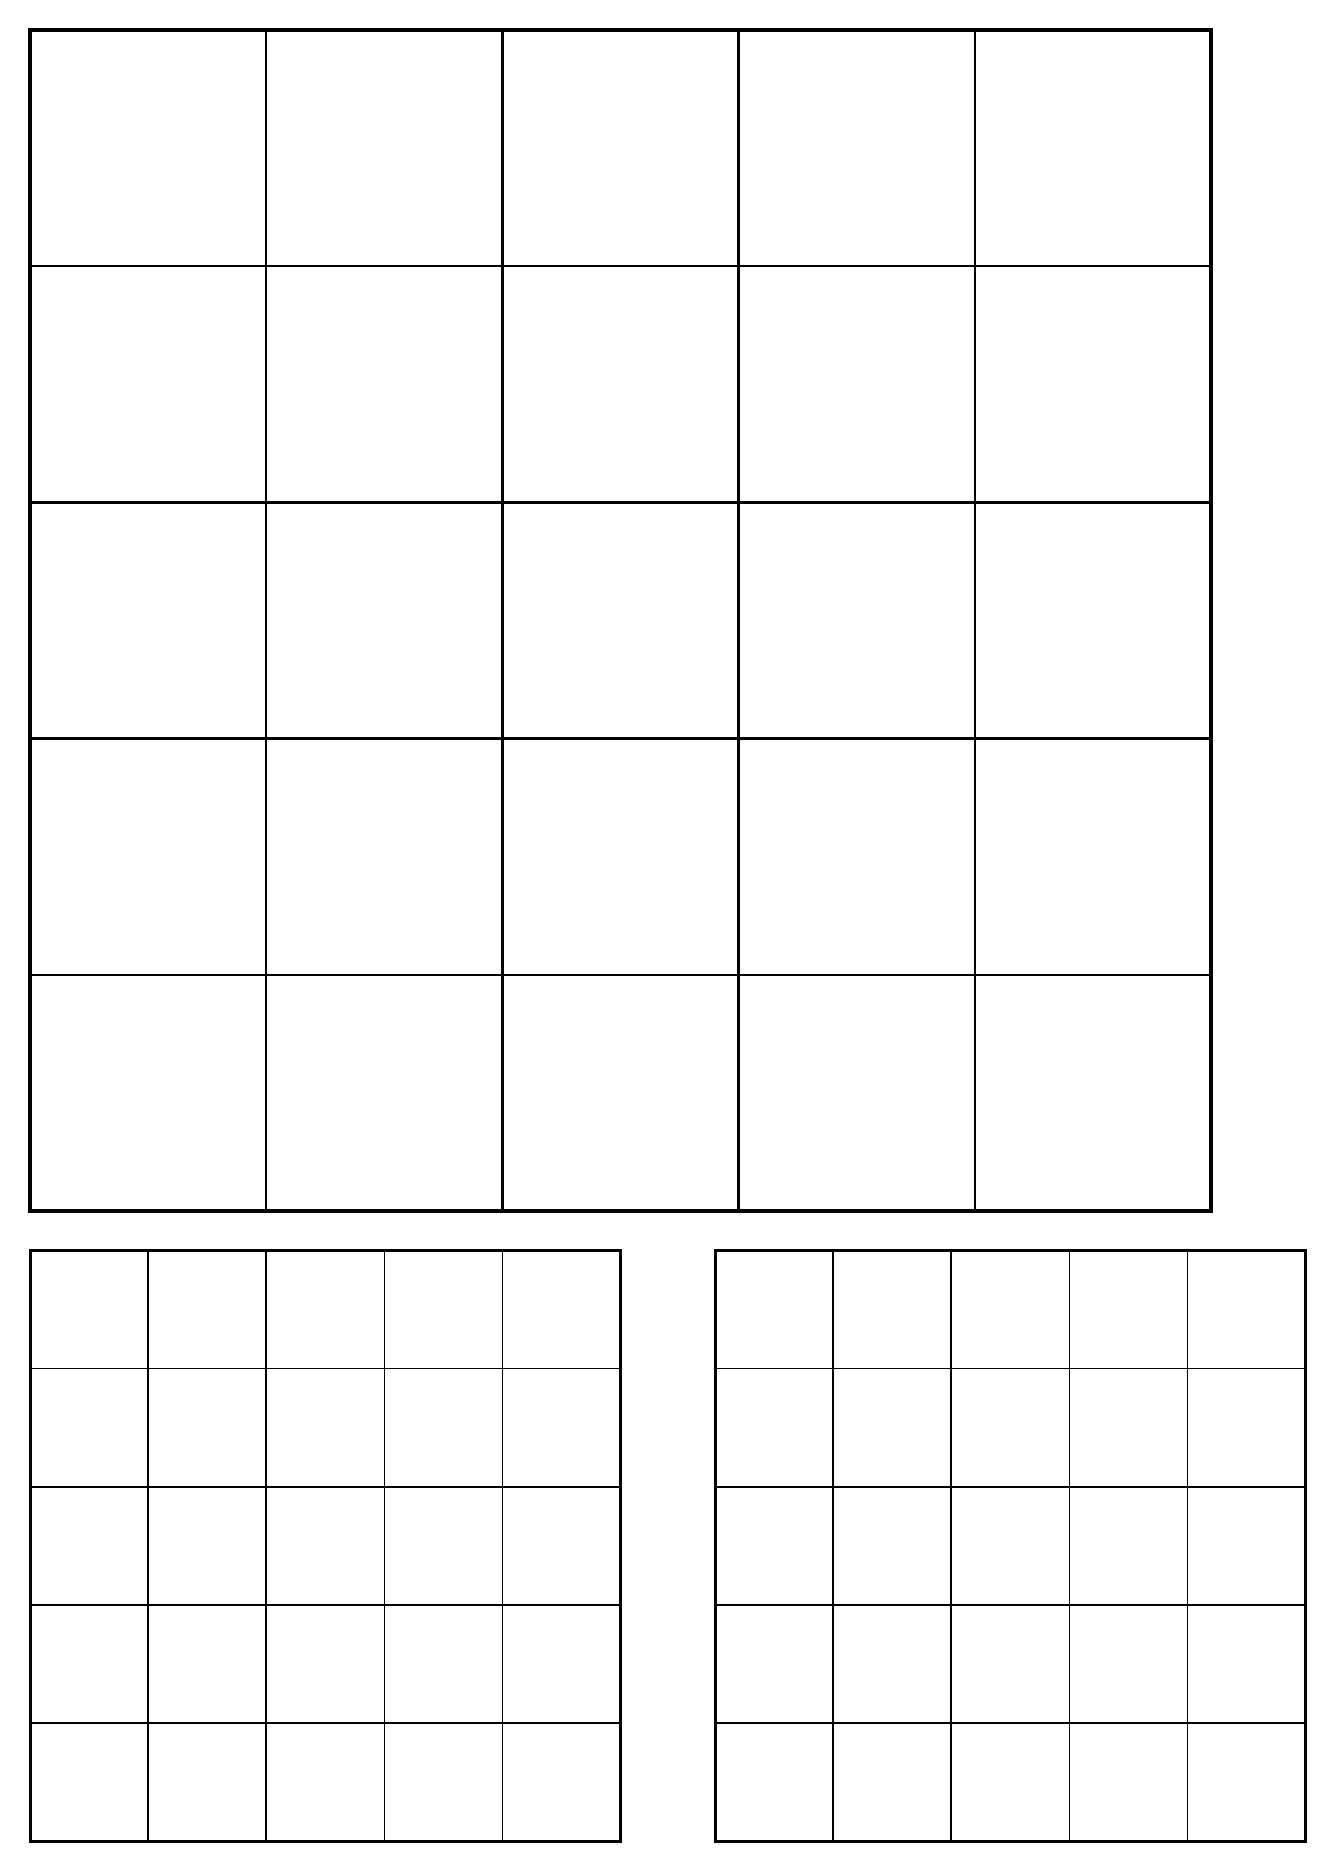
\begin{tikzpicture}[x=1mm,y=1mm,line cap=rect]
\draw[line width=0.9pt] (30,0) -- (30,-150);
\draw[line width=0.9pt] (60,0) -- (60,-150);
\draw[line width=0.9pt] (90,0) -- (90,-150);
\draw[line width=0.9pt] (120,0) -- (120,-150);
\draw[line width=0.9pt] (0,-30) -- (150,-30);
\draw[line width=0.9pt] (0,-60) -- (150,-60);
\draw[line width=0.9pt] (0,-90) -- (150,-90);
\draw[line width=0.9pt] (0,-120) -- (150,-120);
\draw[line width=1.7pt] (0,0) rectangle (150,-150);
\draw[line width=0.6pt] (15,-155) -- (15,-230);
\draw[line width=0.6pt] (30,-155) -- (30,-230);
\draw[line width=0.6pt] (45,-155) -- (45,-230);
\draw[line width=0.6pt] (60,-155) -- (60,-230);
\draw[line width=0.6pt] (0,-170) -- (75,-170);
\draw[line width=0.6pt] (0,-185) -- (75,-185);
\draw[line width=0.6pt] (0,-200) -- (75,-200);
\draw[line width=0.6pt] (0,-215) -- (75,-215);
\draw[line width=1.1pt] (0,-155) rectangle (75,-230);
\draw[line width=0.6pt] (102,-155) -- (102,-230);
\draw[line width=0.6pt] (117,-155) -- (117,-230);
\draw[line width=0.6pt] (132,-155) -- (132,-230);
\draw[line width=0.6pt] (147,-155) -- (147,-230);
\draw[line width=0.6pt] (87,-170) -- (162,-170);
\draw[line width=0.6pt] (87,-185) -- (162,-185);
\draw[line width=0.6pt] (87,-200) -- (162,-200);
\draw[line width=0.6pt] (87,-215) -- (162,-215);
\draw[line width=1.1pt] (87,-155) rectangle (162,-230);
\end{tikzpicture}

\newpage
\textbf{Problem 6:} Fill each strip with as few seeds as you can, and draw the seeds.\par\vspace{5mm}
\noindent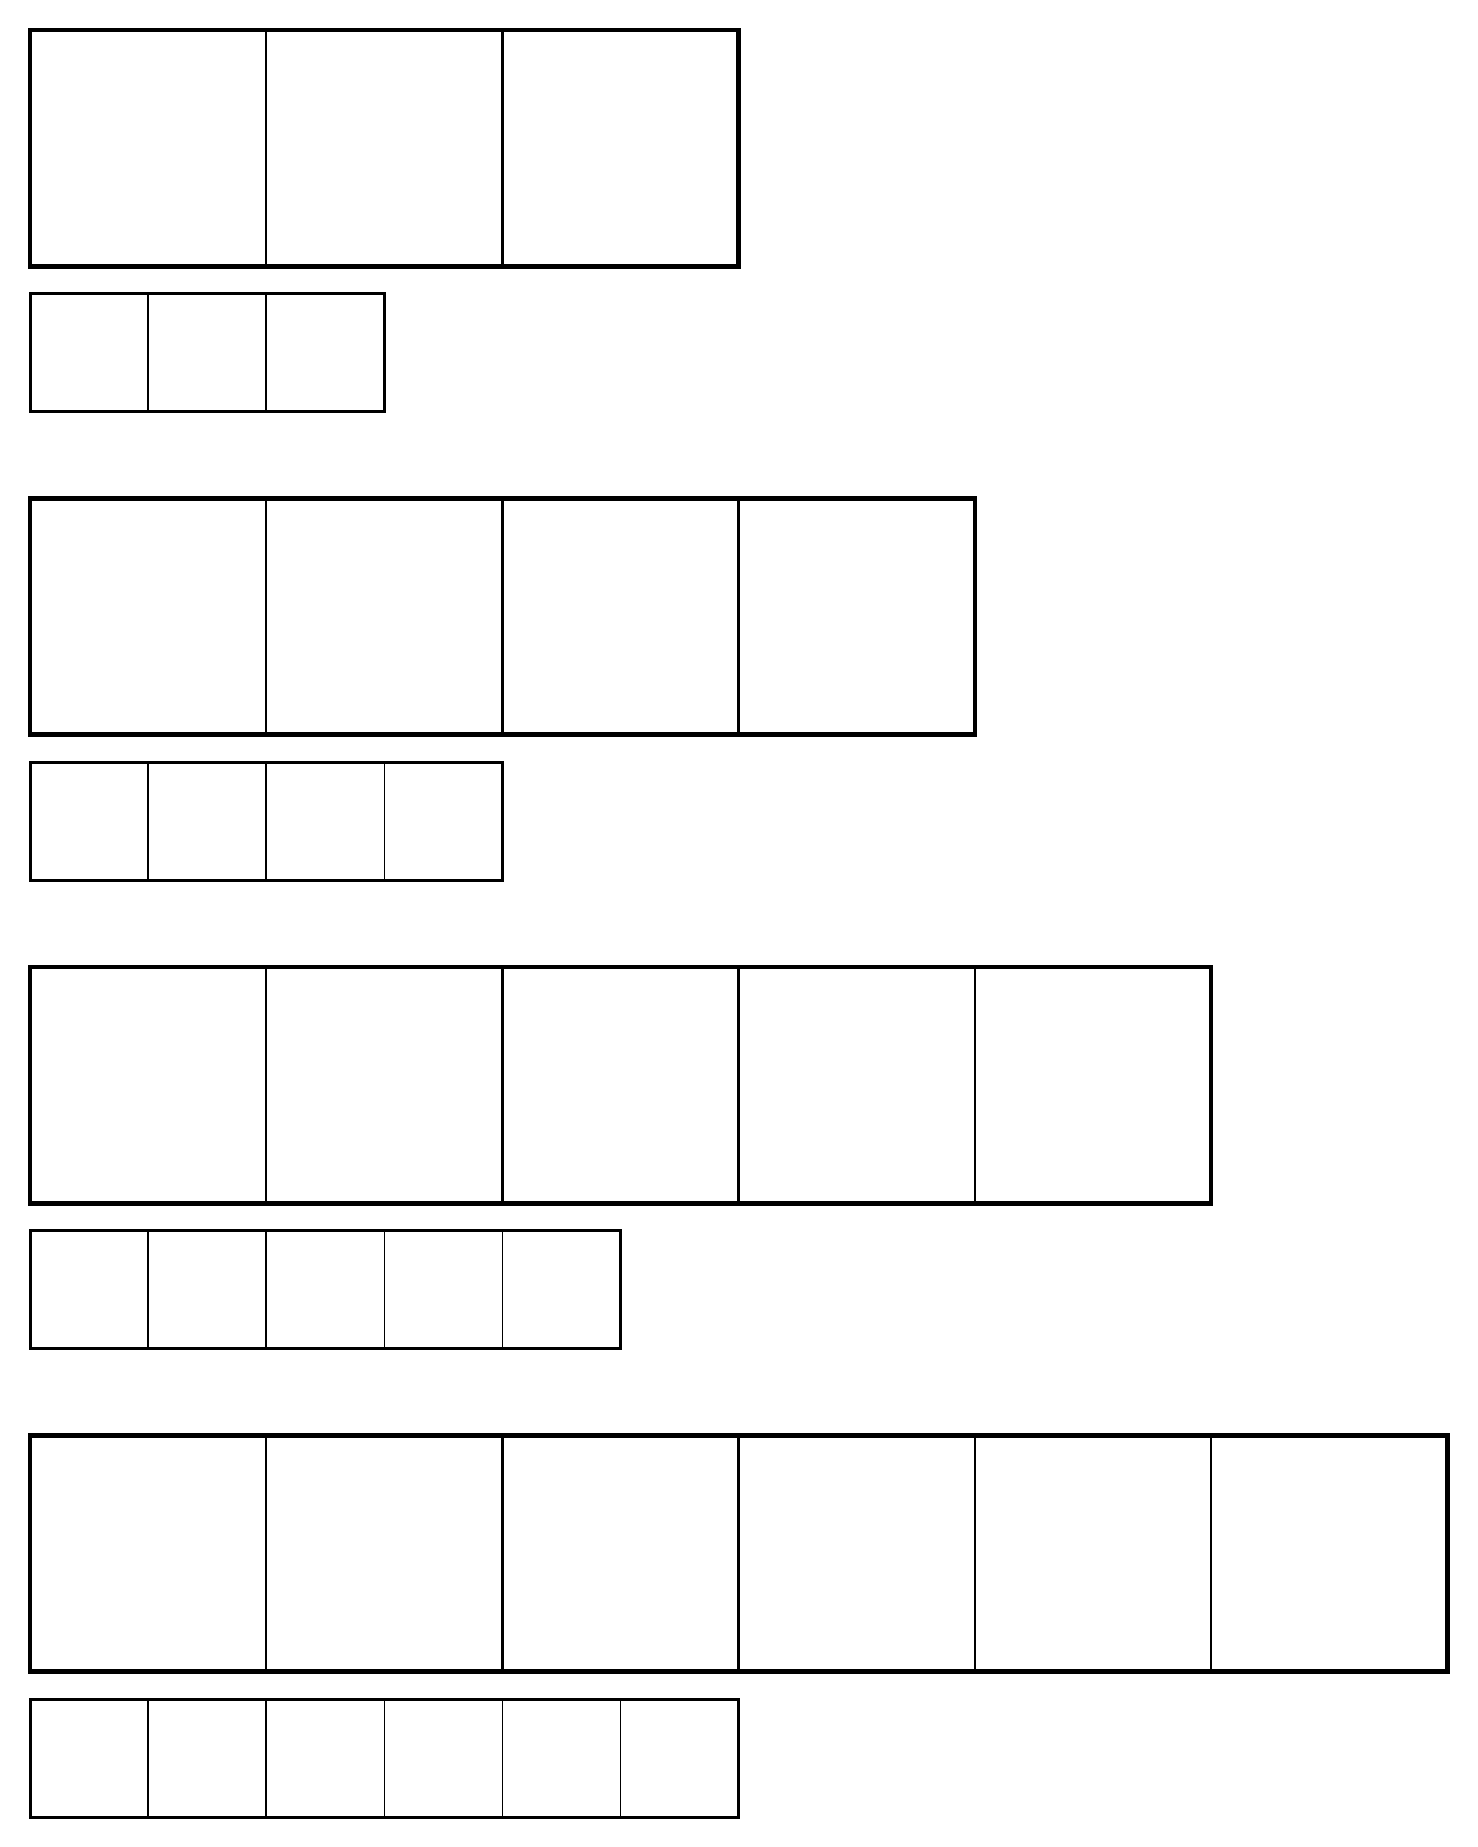
\begin{tikzpicture}[x=1mm,y=1mm,line cap=rect]
\draw[line width=0.9pt] (30,0) -- (30,-30);
\draw[line width=0.9pt] (60,0) -- (60,-30);
\draw[line width=1.7pt] (0,0) rectangle (90,-30);
\draw[line width=0.6pt] (15,-33.5) -- (15,-48.5);
\draw[line width=0.6pt] (30,-33.5) -- (30,-48.5);
\draw[line width=1.1pt] (0,-33.5) rectangle (45,-48.5);
\draw[line width=0.9pt] (30,-59.5) -- (30,-89.5);
\draw[line width=0.9pt] (60,-59.5) -- (60,-89.5);
\draw[line width=0.9pt] (90,-59.5) -- (90,-89.5);
\draw[line width=1.7pt] (0,-59.5) rectangle (120,-89.5);
\draw[line width=0.6pt] (15,-93.0) -- (15,-108.0);
\draw[line width=0.6pt] (30,-93.0) -- (30,-108.0);
\draw[line width=0.6pt] (45,-93.0) -- (45,-108.0);
\draw[line width=1.1pt] (0,-93.0) rectangle (60,-108.0);
\draw[line width=0.9pt] (30,-119.0) -- (30,-149.0);
\draw[line width=0.9pt] (60,-119.0) -- (60,-149.0);
\draw[line width=0.9pt] (90,-119.0) -- (90,-149.0);
\draw[line width=0.9pt] (120,-119.0) -- (120,-149.0);
\draw[line width=1.7pt] (0,-119.0) rectangle (150,-149.0);
\draw[line width=0.6pt] (15,-152.5) -- (15,-167.5);
\draw[line width=0.6pt] (30,-152.5) -- (30,-167.5);
\draw[line width=0.6pt] (45,-152.5) -- (45,-167.5);
\draw[line width=0.6pt] (60,-152.5) -- (60,-167.5);
\draw[line width=1.1pt] (0,-152.5) rectangle (75,-167.5);
\draw[line width=0.9pt] (30,-178.5) -- (30,-208.5);
\draw[line width=0.9pt] (60,-178.5) -- (60,-208.5);
\draw[line width=0.9pt] (90,-178.5) -- (90,-208.5);
\draw[line width=0.9pt] (120,-178.5) -- (120,-208.5);
\draw[line width=0.9pt] (150,-178.5) -- (150,-208.5);
\draw[line width=1.7pt] (0,-178.5) rectangle (180,-208.5);
\draw[line width=0.6pt] (15,-212.0) -- (15,-227.0);
\draw[line width=0.6pt] (30,-212.0) -- (30,-227.0);
\draw[line width=0.6pt] (45,-212.0) -- (45,-227.0);
\draw[line width=0.6pt] (60,-212.0) -- (60,-227.0);
\draw[line width=0.6pt] (75,-212.0) -- (75,-227.0);
\draw[line width=1.1pt] (0,-212.0) rectangle (90,-227.0);
\end{tikzpicture}

\newpage
\textbf{Problem 7:} Fill each board with as few seeds as you can, and draw the seeds.\par\vspace{5mm}
\noindent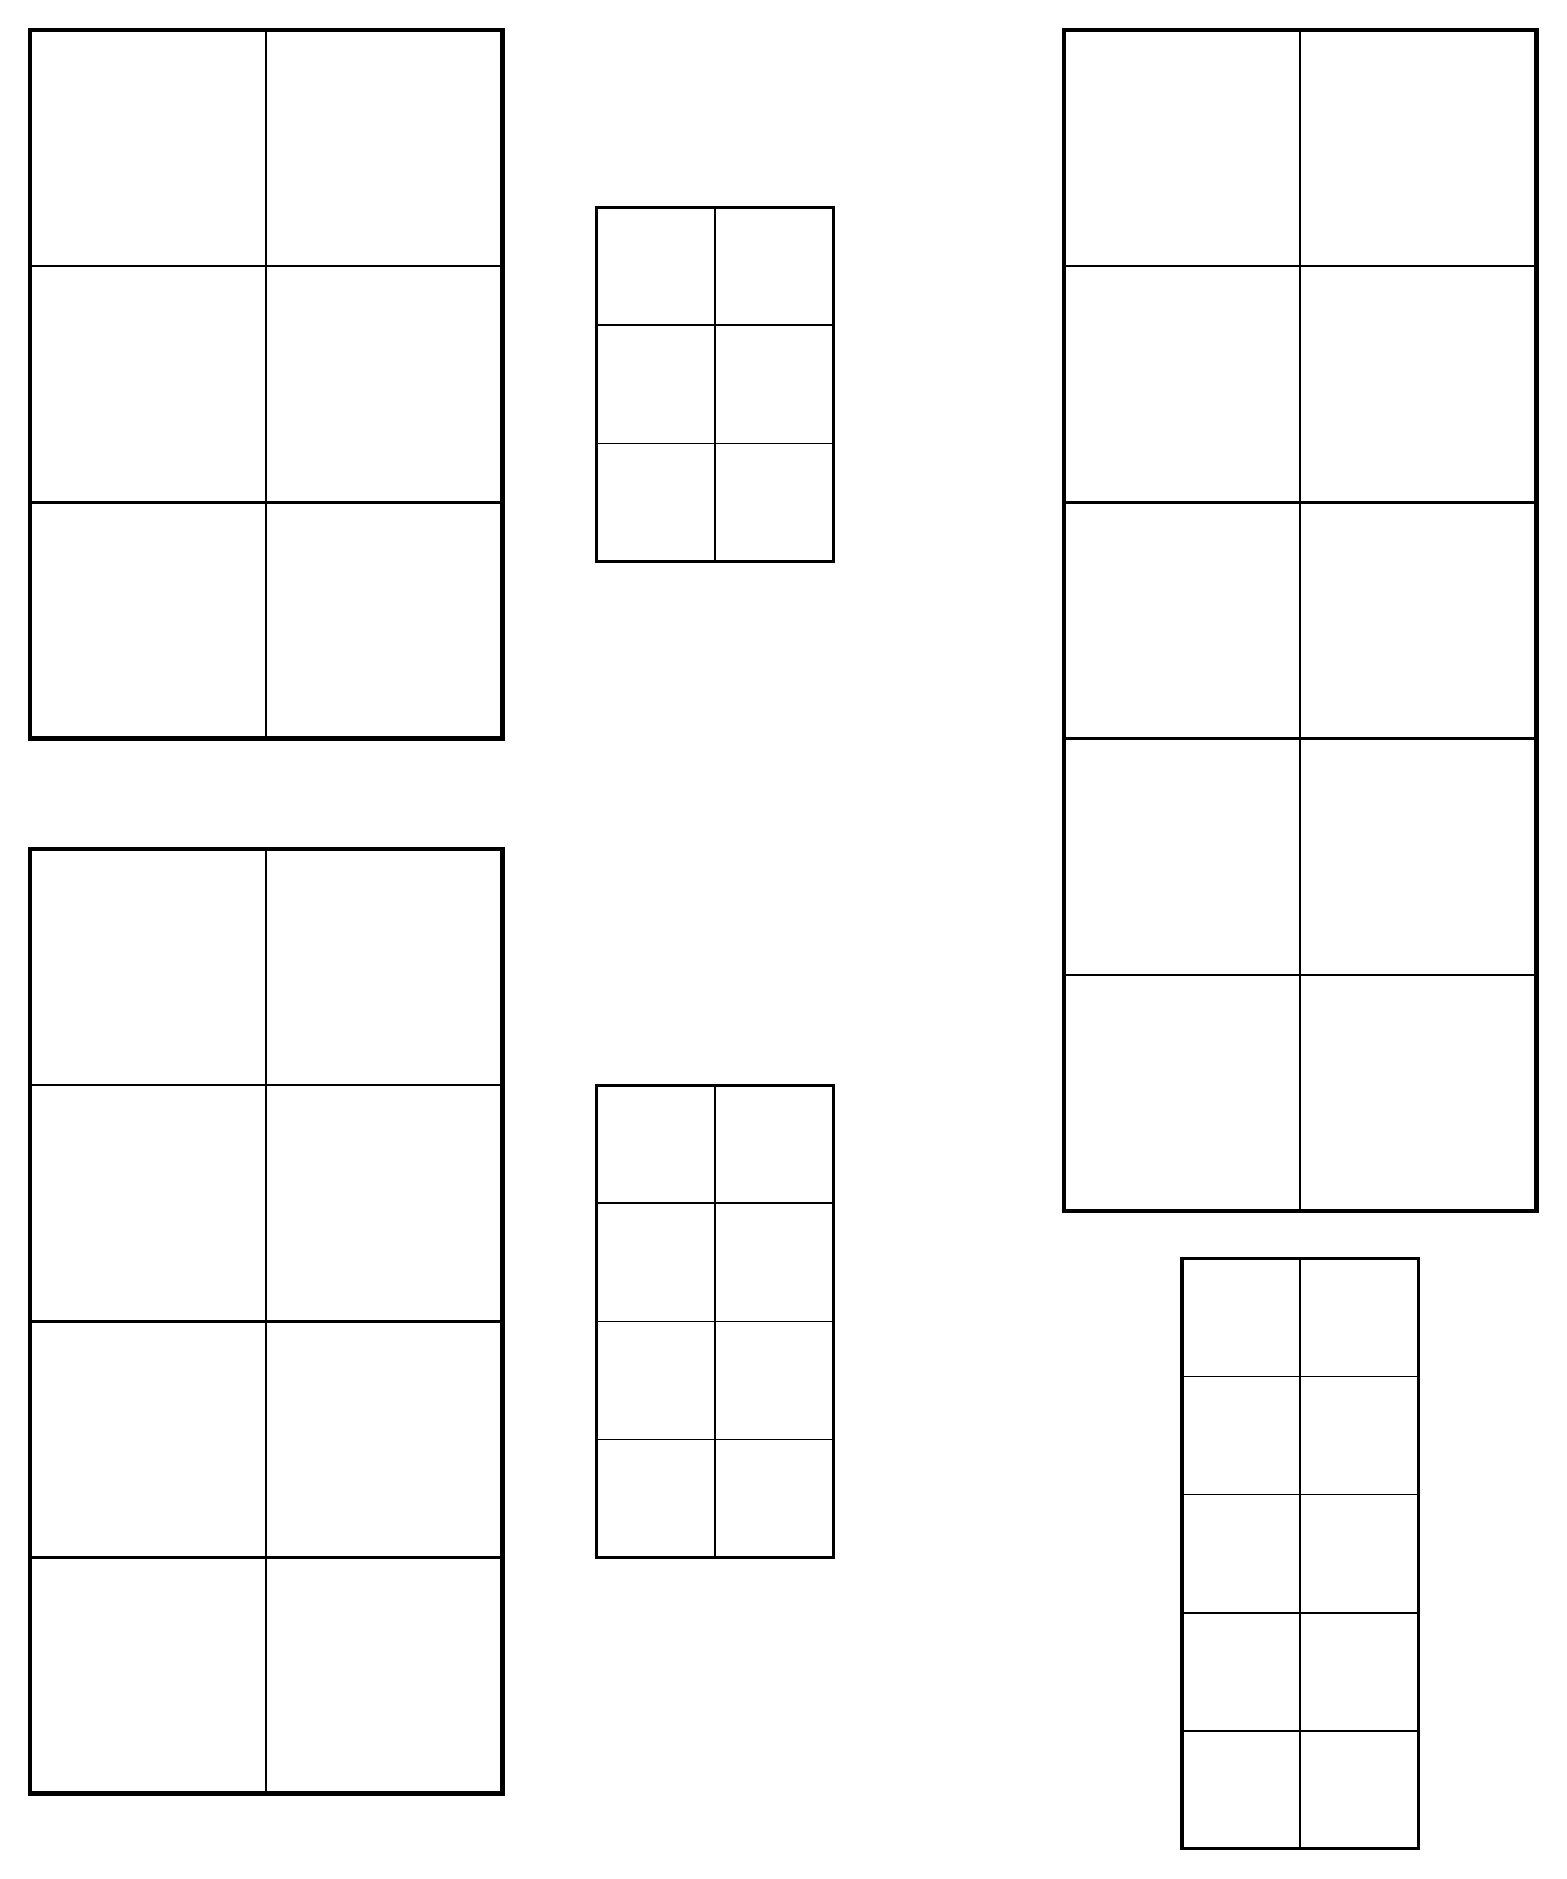
\begin{tikzpicture}[x=1mm,y=1mm,line cap=rect]
\draw[line width=0.9pt] (30,0) -- (30,-90);
\draw[line width=0.9pt] (0,-30) -- (60,-30);
\draw[line width=0.9pt] (0,-60) -- (60,-60);
\draw[line width=1.7pt] (0,0) rectangle (60,-90);
\draw[line width=0.6pt] (87,-22.5) -- (87,-67.5);
\draw[line width=0.6pt] (72,-37.5) -- (102,-37.5);
\draw[line width=0.6pt] (72,-52.5) -- (102,-52.5);
\draw[line width=1.1pt] (72,-22.5) rectangle (102,-67.5);
\draw[line width=0.9pt] (30,-104) -- (30,-224);
\draw[line width=0.9pt] (0,-134) -- (60,-134);
\draw[line width=0.9pt] (0,-164) -- (60,-164);
\draw[line width=0.9pt] (0,-194) -- (60,-194);
\draw[line width=1.7pt] (0,-104) rectangle (60,-224);
\draw[line width=0.6pt] (87,-134.0) -- (87,-194.0);
\draw[line width=0.6pt] (72,-149.0) -- (102,-149.0);
\draw[line width=0.6pt] (72,-164.0) -- (102,-164.0);
\draw[line width=0.6pt] (72,-179.0) -- (102,-179.0);
\draw[line width=1.1pt] (72,-134.0) rectangle (102,-194.0);
\draw[line width=0.9pt] (161.3,0) -- (161.3,-150);
\draw[line width=0.9pt] (131.3,-30) -- (191.3,-30);
\draw[line width=0.9pt] (131.3,-60) -- (191.3,-60);
\draw[line width=0.9pt] (131.3,-90) -- (191.3,-90);
\draw[line width=0.9pt] (131.3,-120) -- (191.3,-120);
\draw[line width=1.7pt] (131.3,0) rectangle (191.3,-150);
\draw[line width=0.6pt] (161.3,-156) -- (161.3,-231);
\draw[line width=0.6pt] (146.3,-171) -- (176.3,-171);
\draw[line width=0.6pt] (146.3,-186) -- (176.3,-186);
\draw[line width=0.6pt] (146.3,-201) -- (176.3,-201);
\draw[line width=0.6pt] (146.3,-216) -- (176.3,-216);
\draw[line width=1.1pt] (146.3,-156) rectangle (176.3,-231);
\end{tikzpicture}

\newpage
\textbf{Problem 8:} Put seeds on the dots of one board. Ring each seed that can come off by itself while the other seeds still fill the board. Put each seed back before you try the next one.\par\vspace{5mm}
\noindent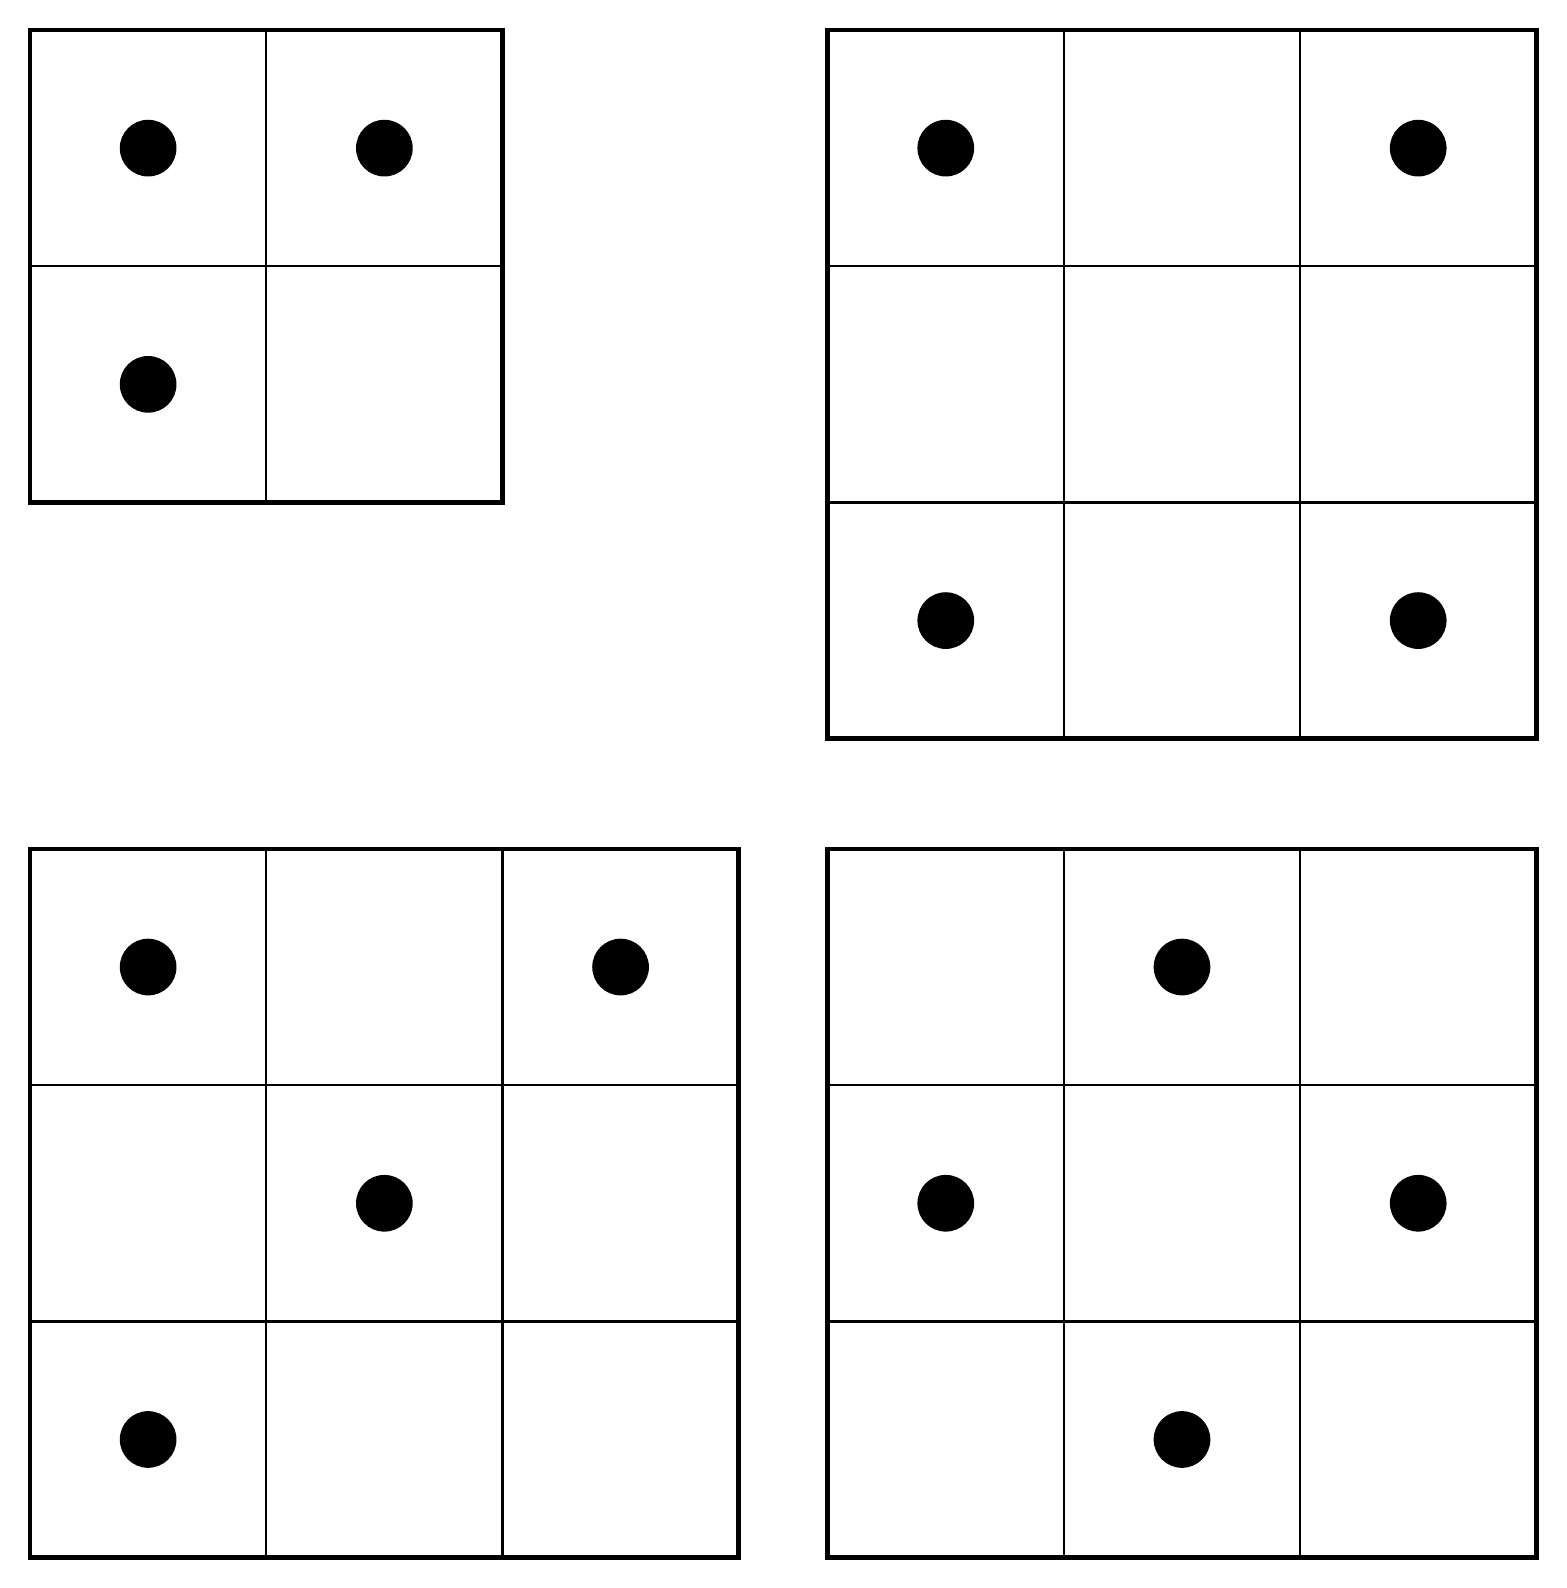
\begin{tikzpicture}[x=1mm,y=1mm,line cap=rect]
\draw[line width=0.9pt] (30,0) -- (30,-60);
\draw[line width=0.9pt] (0,-30) -- (60,-30);
\draw[line width=1.7pt] (0,0) rectangle (60,-60);
\fill (15.00,-15.00) circle (3.6);
\fill (45.00,-15.00) circle (3.6);
\fill (15.00,-45.00) circle (3.6);
\draw[line width=0.9pt] (131.3,0) -- (131.3,-90);
\draw[line width=0.9pt] (161.3,0) -- (161.3,-90);
\draw[line width=0.9pt] (101.30000000000001,-30) -- (191.3,-30);
\draw[line width=0.9pt] (101.30000000000001,-60) -- (191.3,-60);
\draw[line width=1.7pt] (101.30000000000001,0) rectangle (191.3,-90);
\fill (116.30,-15.00) circle (3.6);
\fill (176.30,-15.00) circle (3.6);
\fill (116.30,-75.00) circle (3.6);
\fill (176.30,-75.00) circle (3.6);
\draw[line width=0.9pt] (30,-104) -- (30,-194);
\draw[line width=0.9pt] (60,-104) -- (60,-194);
\draw[line width=0.9pt] (0,-134) -- (90,-134);
\draw[line width=0.9pt] (0,-164) -- (90,-164);
\draw[line width=1.7pt] (0,-104) rectangle (90,-194);
\fill (15.00,-119.00) circle (3.6);
\fill (75.00,-119.00) circle (3.6);
\fill (45.00,-149.00) circle (3.6);
\fill (15.00,-179.00) circle (3.6);
\draw[line width=0.9pt] (131.3,-104) -- (131.3,-194);
\draw[line width=0.9pt] (161.3,-104) -- (161.3,-194);
\draw[line width=0.9pt] (101.30000000000001,-134) -- (191.3,-134);
\draw[line width=0.9pt] (101.30000000000001,-164) -- (191.3,-164);
\draw[line width=1.7pt] (101.30000000000001,-104) rectangle (191.3,-194);
\fill (146.30,-119.00) circle (3.6);
\fill (116.30,-149.00) circle (3.6);
\fill (176.30,-149.00) circle (3.6);
\fill (146.30,-179.00) circle (3.6);
\end{tikzpicture}

\newpage
\textbf{Problem 9:} Put seeds on the dots. Take seeds off one at a time while the board still fills. Draw the seeds left when no more can go. Can you end with a different number of seeds?\par\vspace{5mm}
\noindent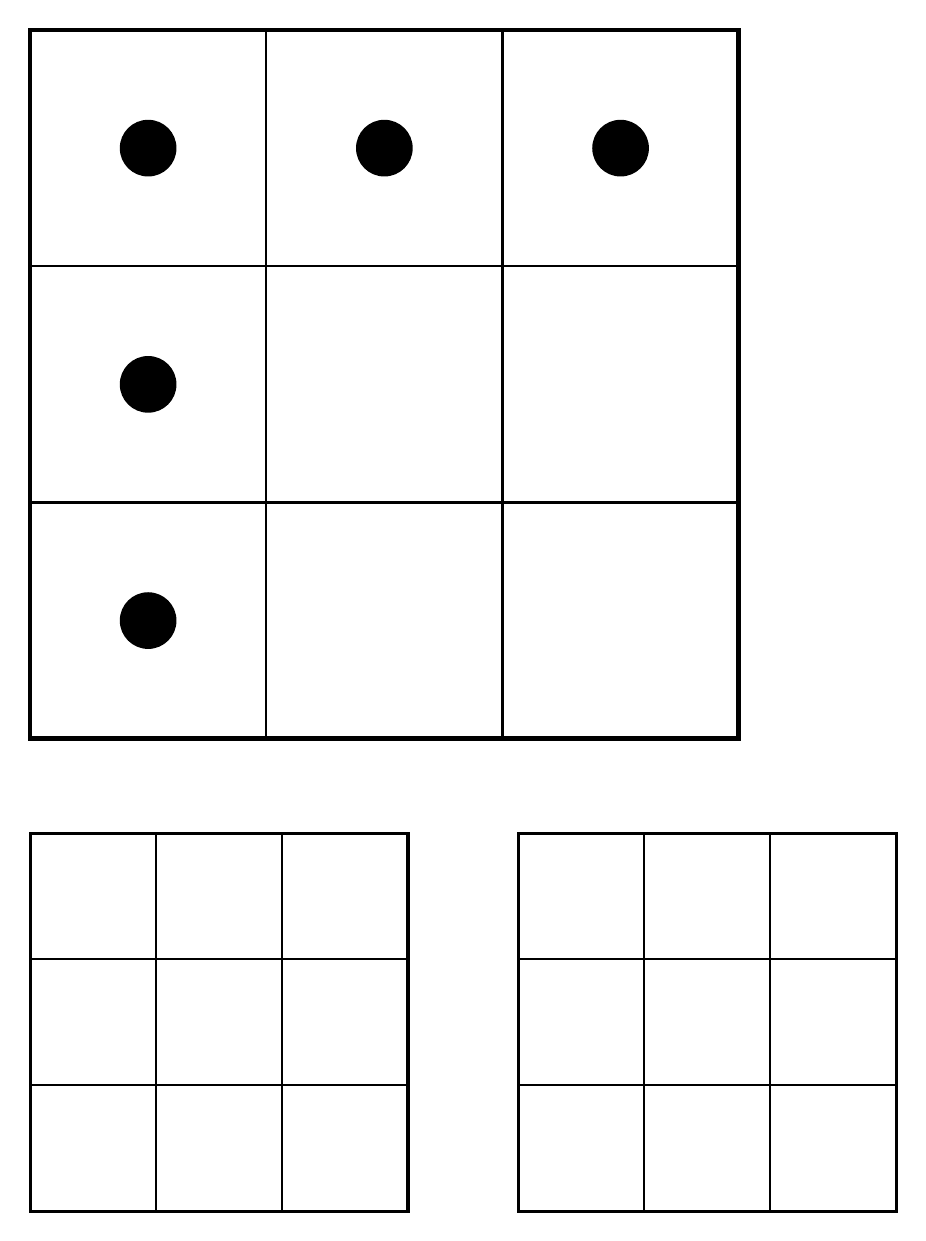
\begin{tikzpicture}[x=1mm,y=1mm,line cap=rect]
\draw[line width=0.9pt] (30,0) -- (30,-90);
\draw[line width=0.9pt] (60,0) -- (60,-90);
\draw[line width=0.9pt] (0,-30) -- (90,-30);
\draw[line width=0.9pt] (0,-60) -- (90,-60);
\draw[line width=1.7pt] (0,0) rectangle (90,-90);
\fill (15.00,-15.00) circle (3.6);
\fill (45.00,-15.00) circle (3.6);
\fill (75.00,-15.00) circle (3.6);
\fill (15.00,-45.00) circle (3.6);
\fill (15.00,-75.00) circle (3.6);
\draw[line width=0.6pt] (16,-102) -- (16,-150);
\draw[line width=0.6pt] (32,-102) -- (32,-150);
\draw[line width=0.6pt] (0,-118) -- (48,-118);
\draw[line width=0.6pt] (0,-134) -- (48,-134);
\draw[line width=1.1pt] (0,-102) rectangle (48,-150);
\draw[line width=0.6pt] (78,-102) -- (78,-150);
\draw[line width=0.6pt] (94,-102) -- (94,-150);
\draw[line width=0.6pt] (62,-118) -- (110,-118);
\draw[line width=0.6pt] (62,-134) -- (110,-134);
\draw[line width=1.1pt] (62,-102) rectangle (110,-150);
\end{tikzpicture}

\end{document}
